\section{Relevant terms} \label{appendix:terms}
\begin{itemize}
	\item[] \textbf{Abstract place (AP)}: A point in space or area non-conforming to current or historical ABs or recognized POIs.
	\item[] \textbf{Administrative boundary (AB)}: A geographical area limit managed by an entity; ex: the municipality of Lisbon, Portugal or the 2nd congressional district in Colorado .
	\item[] \textbf{Attribute}: an informative element of data stored in a data field. 
	\begin{itemize}
		\item[] \textbf{Spatial Attribute (SA)}: a description relating to location; ex: ‘where did something happen’ or ‘where was it logged’.
		\item[] \textbf{Temporal Attribute (TA)}: a description of when; ex: ‘at what time did it happen’ or ‘which day was it published’. 
		\item[] \textbf{Thematic Attribute (ThA)}: a description of what, why, or how; ex: ‘what happened’ or ‘who published it’).
	\end{itemize}
	\item[] \textbf{Comma separated value (CSV)}: text file of data records (features) in which each record is stored as a new line and its attributes (fields) are delimited by a comma.
	\item[] \textbf{Data model}: a graphical representation of the data structure and relationships definitions.
	\item[] \textbf{Gazetteer}: A geographical index relating descriptors to location; ex: \href{https://www.geonames.org/}{GeoNames} , which related names of places to geographical coordinates.
	\item[] \textbf{Geographic information system (GIS)}: A framework for the manipulation and analysis of geographic data.
	\item[] \textbf{Incident}: Defined within the project as any content of a news article that has spatial and temporal dimensions.  These can be past, present, future, or related to multiple instances in time. Likewise, each can occur in a single place or in multiple places, as a point in space or as an area (polygon), and be associated with a recognizable place (such as an AB or a POI) or over areas not commonly recognized (an AP).
	\item[] \textbf{Open source (OS)}: a development methodology, the product of which is free of any restrictions of use, permits access to (for the study or modification of) the source code as well as the distribution of original or modified copies to third parties.
	\item[] \textbf{Point of Interest (POI)}: any entity (natural or artificial) with a well-defined location; ex: Praça do Comércio or Garden of the Gods.
	\item[] \textbf{Proof of concept (POC)}: functional or demonstrative of the basic project concepts.
	\item[] \textbf{Tag}: content, section, or descriptive designations defined by the media publisher; ex: ‘política’, ‘primeiro-ministro’, ‘governo’ (from Público), or ‘coronavirus’, ‘denver’, ‘homelessness’ (from The Denver Post).
	\item[] \textbf{User interface (UI)}: the method of interaction between a user and the program.
	\item[] \textbf{Web application (Web App)}: a program running on a web server that is accessible via a web browser with internet connectivity.
	\item[] \textbf{Wireframe}: a design mockup of a website to demonstrate functional logic.
\end{itemize}

\newpage
\section{Preliminary specification} \label{appendix:organization}
\begin{figure}[H]
	\centering
	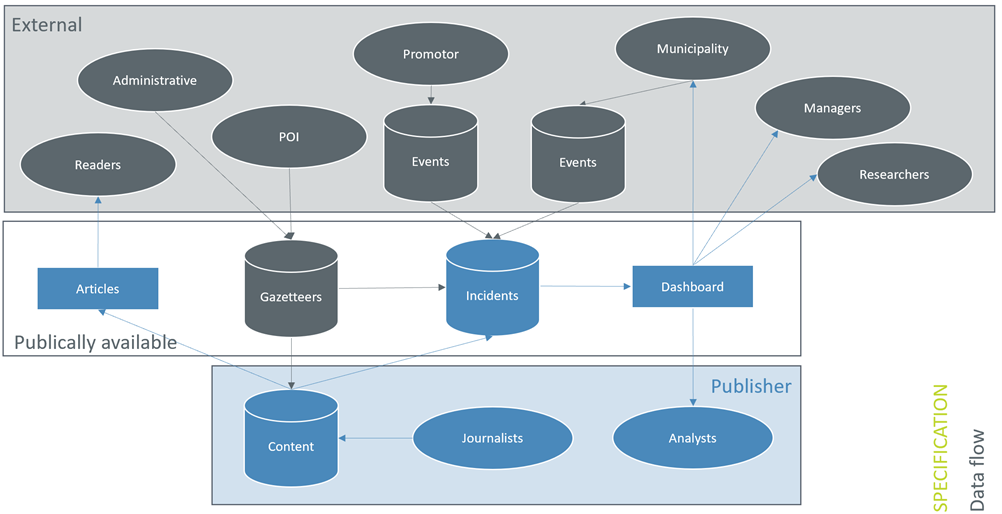
\includegraphics[width=.9\linewidth]{images/information_flow.png}
	\caption{Preliminary data and information flow}
	\label{fig:info_flow}
\end{figure}

\begin{figure}[H]
	\centering
	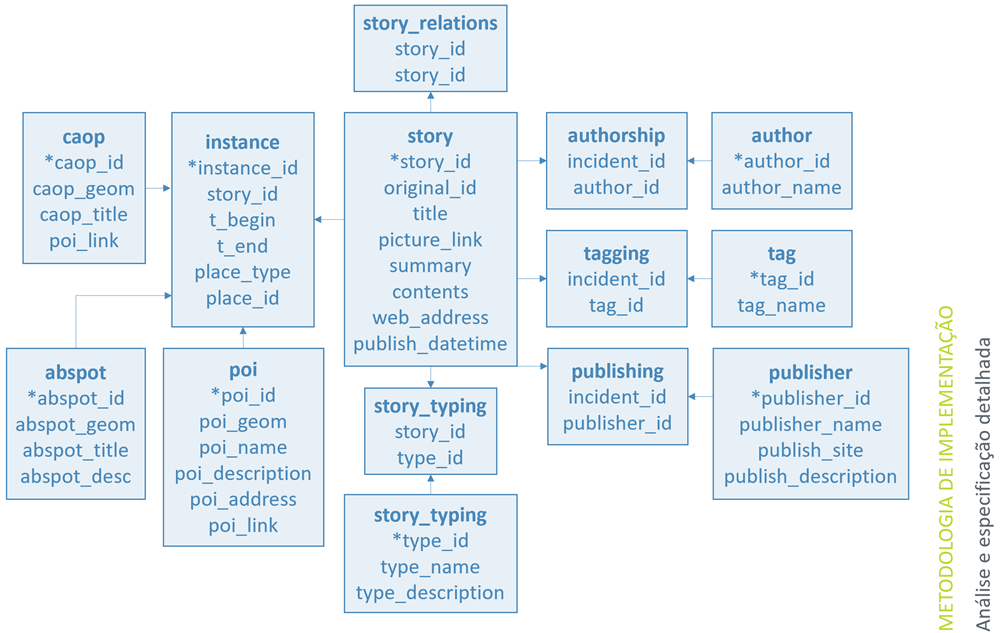
\includegraphics[width=.9\linewidth]{images/data_model.png}
	\caption{Preliminary data model fo the spatial database}
	\label{fig:data_model}
\end{figure}

\begin{figure}[H]
	\centering
	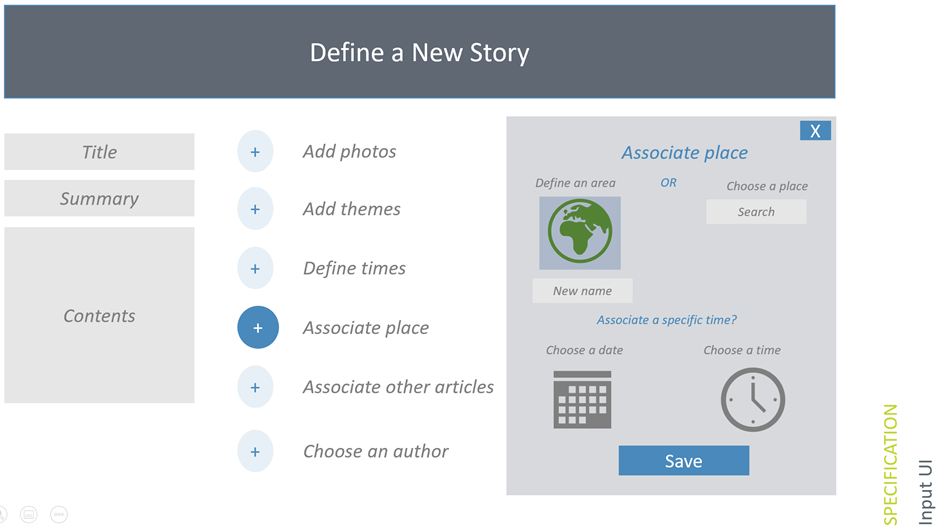
\includegraphics[width=.9\linewidth]{images/input_layout.png}
	\caption{Preliminary \textit{Input} layout}
	\label{fig:input_ui}
\end{figure}

\begin{figure}[H]
	\centering
	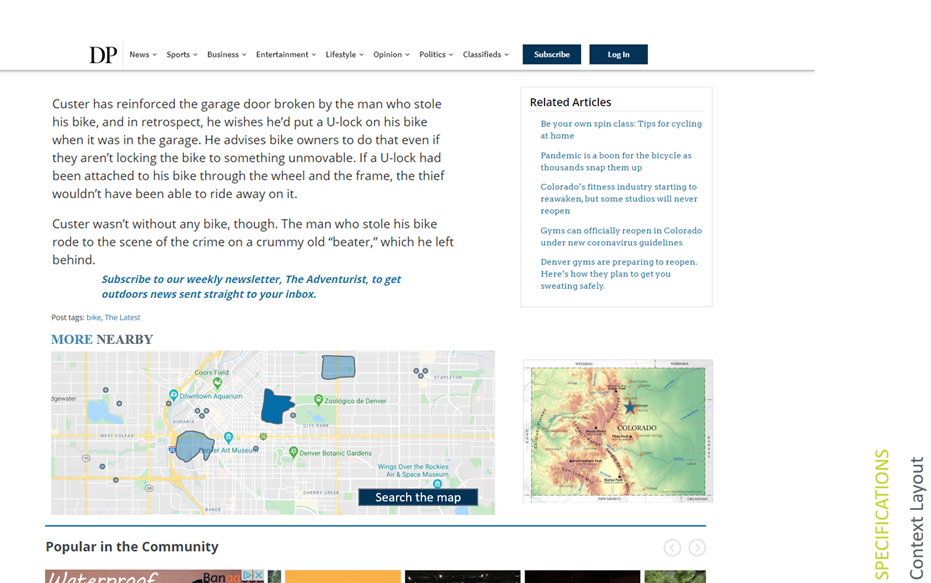
\includegraphics[width=.9\linewidth]{images/context_layout.png}
	\caption{Preliminary \textit{Context} layout}
	\label{fig:context_ui}
\end{figure}

\begin{figure}[H]
	\centering
	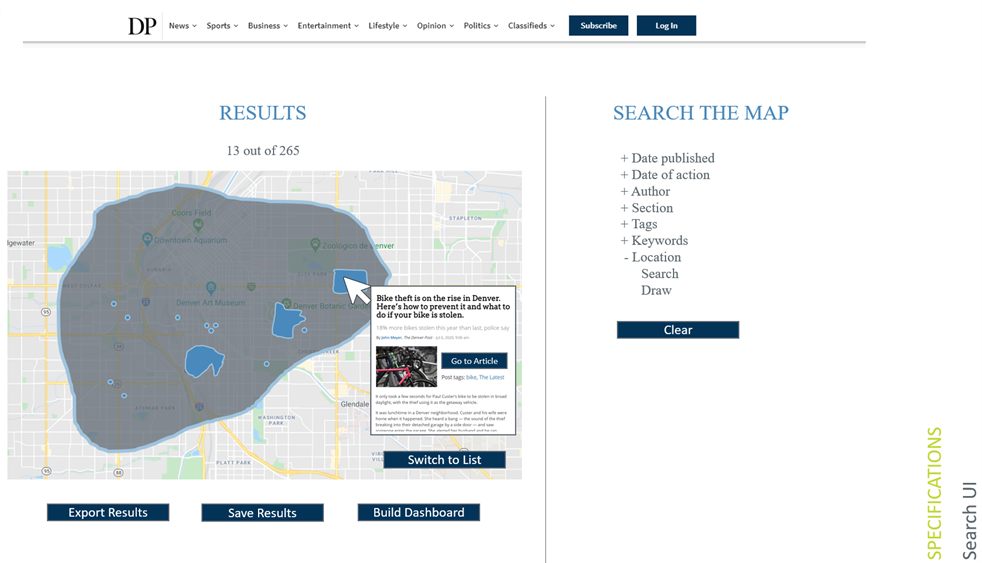
\includegraphics[width=.9\linewidth]{images/search_layout.png}
	\caption{Preliminary \textit{Search} layout}
	\label{fig:search_ui}
\end{figure}

\begin{figure}[H]
	\centering
	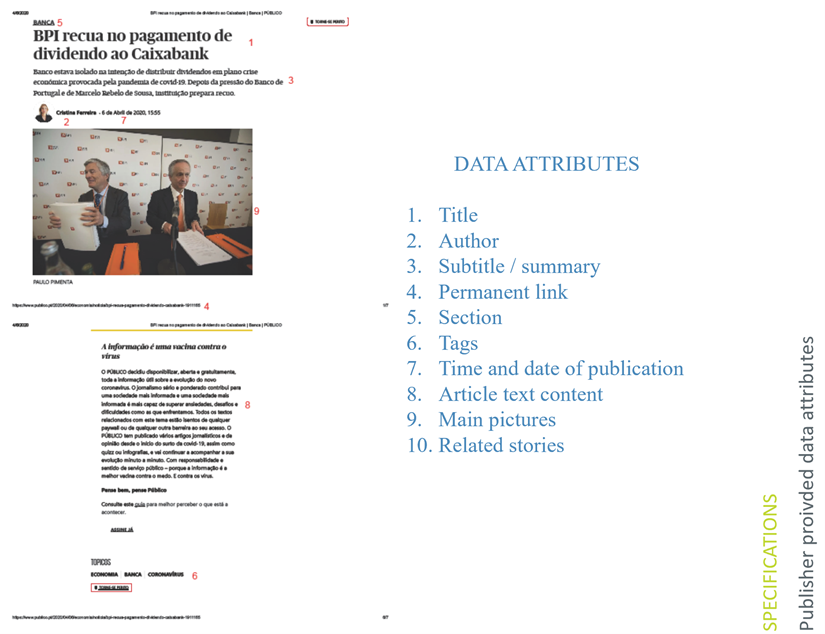
\includegraphics[width=.9\linewidth]{images/provided_attributes.png}
	\caption{Publisher provided data attributes}
	\label{fig:publisher_atts}
\end{figure}

%{\color{red} Include specifications matrix}

\newpage
\section{Existing efforts}\label{appendix:existing_projects}
Some projects are already mining place (as well as other attributes) from existing data lakes of publication data to provide geospatial and temporal distributions. One such effort is \href{https://www.gdeltproject.org/}{The GDELT Project}, which extracts place as well as actors, sentiment, and event connection (among other elements) from journalistic media across the globe, including publications from as far back as 1979. This and similar projects are powerful and hugely informative, especially as they apply to existing published data. The proposed project should leverage such tools for the inclusion of historic data into the developed database for investigation into the past (already published) incidents. 

However, the existing automated extraction includes several challenges:
\begin{enumerate}
	\item It is not yet perfect, and places may be misattributed (Lisbon, Ohio in the USA may be accidentally attributed to Lisbon, Portugal).
	\item It does not support the subtlety of incidents occurring in non-conforming places (an incident may not apply to a single administrative boundary but really fall into a subsection of one or several).
	\item It requires technical prowess and tools to explore the data. A user is unable to define a spatial area of interest (such as their route to work with a half mile buffer or some other irregular shape) and search for all spatially related results, nor it is easy to apply temporal or thematic attributes without prior experience querying results. 
\end{enumerate}

Therefore, this project offers a functionality specific to the defined user types of news publication services and provides an appropriate user experience to these.

\newpage
\section{Relevant coursework}
\begin{itemize}
	\item{} Cartographic sciences
	\item{} Geographic information standards
	\item{} Geospatial intelligence (GEOINT)
	\item{} Geo-statistics
	\item{} Geospatial data mining
	\item{} Modeling in GIS
	\item{} GIS in organization
	\item{} Open software and programming in GIS
	\item{} Geographic databases and geospatial web services
	\item{} Geographic information system
	\item{} Information technology in cities (I and II)
	\item{} Mobile and ubiquitous computing
	\item{} Sustainable cities
	\item{} Urban analytics
	\item{} Remote sensing
	\item{} Cybersecurity
	\item{} Big data
\end{itemize}